\subsubsubsubsection{Street Factory}
\begin{figure}[h]
\centering
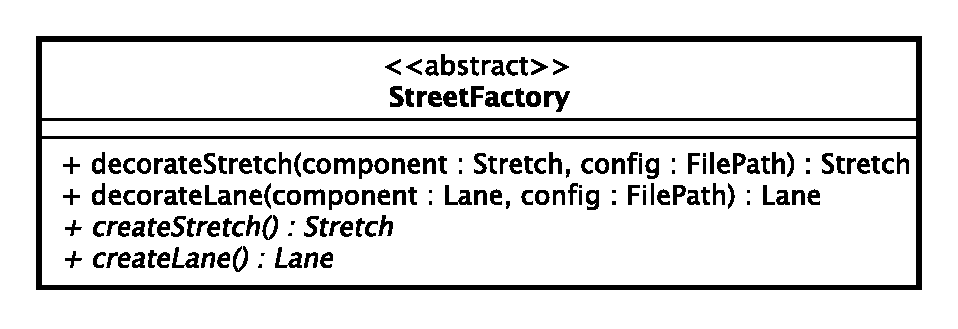
\includegraphics[scale=0.6,keepaspectratio]{images/solution/street_factory.eps}
\caption{App::Reactive::StreetFactory}
\label{fig:sd-app-street-factory}
\end{figure}
\FloatBarrier
\begin{itemize}
  \item \textbf{Description} \\
    It represents the base class of the abstract factory pattern. The 
non-abstract methods of this class are used by StreetBuilder during the
building phase.
  \item \textbf{Operation} \\
  \begin{itemize} 
    \item \texttt{+ decorateStretch(component: Stretch, config: FilePath)} \\
Decorates an existing stretch component according to the information contained
in the configuration file \texttt{config}.
    \item \texttt{+ decorateLane(component: Lane, config: FilePath)} \\
Decorates an existing lane component according to the information contained in
the configuration file \texttt{config}.
    \item \texttt{\textit{+ createStretch() : Stretch}} \\
Abstract method which is intended to create a new stretch component.
    \item \texttt{\textit{+ createLane() : Lane}} \\
Abstract method which is intended to create a new lane component.
  \end{itemize}
\end{itemize}
